\section{SBS-9 down-bending track analysis results from LH2 data}
We are in the process of analyzing all of the LH2 data from SBS-9, replayed in the ``down-bending mode". We have proof that we have something in the order of 39,000 good neutrons detected in HCal, that corresponds to the $p(\gamma,\pi^+)n$ reaction. The more difficult task would be to form the denominator of the efficiency calculation by refining the analysis to cleanly identify the $\pi^+$ events in BigBite that corresponds to the $p(\gamma,\pi^+)n$ reaction with high confidence. Work is ongoing which incorporates PHYTHIA + g4sbs simulations to come up with a set of cut criteria for that. More progress on that will be reported later.

%%%%%%%%%%%%%%%%%%%%%%%%%%%%%%%%%%%%%%%%%%%%%%%%%%%%%%%%%%%%%%%%%%%%%%%%%%%%%%%%%%%%%%%%%%%%%%%%%%%%%%%%%%%%
\subsection{$p(\gamma,\pi^+)n$ event selection exclusively via BigBite}
This will form the ``denominator" of the HCal neutron detection efficiency analysis. Thus it is critically important, that a given event is an exclusive $p(\gamma,\pi^+)n$ event, while making sure that we do not use any data from HCal in this step. That makes this steps quite challenging and it imposes several restrictions on us in what kinematics settings we can reliably perform this analysis, with the 1.5\% momentum resolution of BigBite.

\subsubsection{Event selection criteria using BigBite spectrometer}\label{Denominator cuts}
The following set of cuts are being used for selection of $p(\gamma,\pi^+)n$ events exclusively via BigBite:
\begin{itemize}

    \item Number of GEM hits on a track:
    \begin{verbatim}
        bb.gem.track.nhits[0]>3
    \end{verbatim}

    \item Vertex Z position cut:
    \begin{verbatim}
        abs(bb.tr.vz[0])<0.0725
    \end{verbatim}

    \item The ``End-Point" cut on BigBite track momentum. Explained below in section: \ref{End-point momentum cut}

    \item The photon energy cut. Explained below in section: \ref{Photon energy cut}

    \item HCal active area cut. Explained below in section: \ref{HCal active area cut}.  
    
\end{itemize}

The number of GEM plane hits in track is required to be a minimum of 4 by the first criteria, i.e: at least 4/5 GEM planes in BigBite should have a hit, for the best track, in order for that event to be considered for analysis, which ensures that we are looking at good tracks to some extent. The vertex Z position cut ensures that the all the events being passed are originated from within the Z distance of the target. See figure: \ref{fig:Track_vertex_z_position_cut}. 


\begin{figure}[h!]
    \centering
    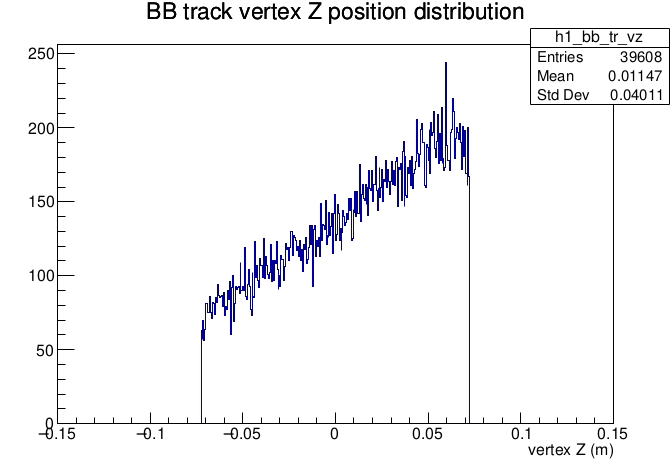
\includegraphics[scale=0.75]{Images/sbs9_hydrogen_analysis/BBTrVzCut.png}
    \caption{Track vertex Z position cut at -7.25 cm and 7.25 cm. The target length is 15 cm}
    \label{fig:Track_vertex_z_position_cut}
\end{figure}

\subsubsection{``End-point" momentum cut}\label{End-point momentum cut}
This cut forms the basis of the physics analysis in the ``end-point" method, by acting as the primary referee in selecting whether a given down-bending track detected in BigBite is from the exclusive single-pion-production channel of $p(\gamma,\pi^+)n$, by filtering out the down-bending tracks that are possibly from multi-pion-production channels, $p(\gamma,\pi^+)N\pi$, or any other processes. The kinematic calculations and principles that lies behind the end-point cuts are explained in the section: \ref{Kinematic calculation}. A lower-bound and an upper-bound cut are being used in analysis for the reconstructed BigBite track momentum variable:
\begin{equation}
    p_{\pi^+}^{limit} (\gamma,\pi) - 0.2 < \texttt{bb.tr.p[0]} < p_{\pi^+}^{max} (\gamma,\pi) + 0.2
\end{equation}
The values $p_{\pi^+}^{limit} (\gamma,\pi)$ and $p_{\pi^+}^{max} (\gamma,\pi)$ are the momentum counterparts of $E_{\pi^+}^{limit} (\gamma,\pi)$ and $E_{\pi^+}^{max} (\gamma,\pi)$, respectively, which are explained in figure: \ref{fig:table4 from GMn proposal}. The upper and lower bounds have been relaxed by 0.2 GeV/c in order to let in more events for the initial analysis but they will be revisited and probably tightened, with the knowledge we get from the PHYTHIA + g4sbs simulation analysis. In this analysis, these threshold values are calculated event-by-event, as they depend on the polar scattering angle $\theta$, using the derivations given in section: \ref{Kinematic calculation}. The effects with and without these polar scattering angle dependent end-point momentum cuts are illustrated in figures: \ref{fig:trp_vs_theta_WithEndPointCuts} and \ref{fig:trp_vs_theta_NoEndPointCuts} respectively. 

\begin{figure}
   \begin{subfigure}{1\textwidth}
        \centering
        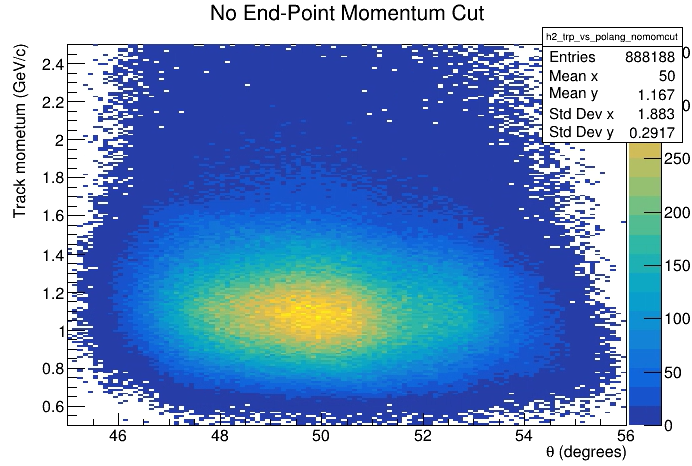
\includegraphics[scale=0.75]{Images/sbs9_hydrogen_analysis/trackP_vs_theta_NoEndPointCut.png}
        \caption{No angle dependent end-point momentum cuts}
        \label{fig:trp_vs_theta_NoEndPointCuts}
   \end{subfigure}
    \hfill
   \begin{subfigure}{1\textwidth}
        \centering
        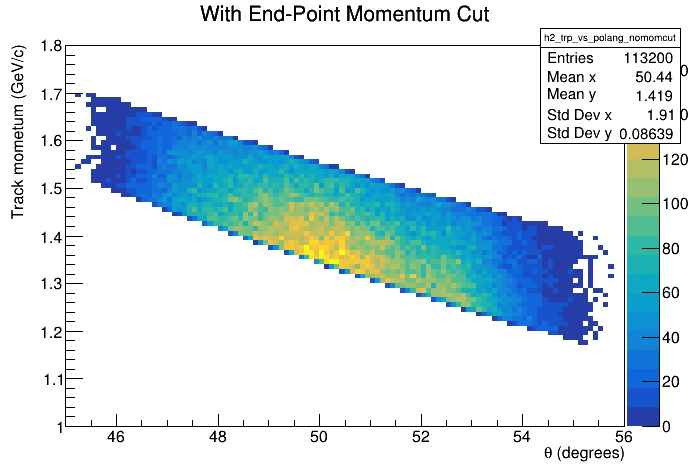
\includegraphics[scale=0.75]{Images/sbs9_hydrogen_analysis/trackP_vs_theta_WithEndPointCut.png}
        \caption{With angle dependent end-point momentum cuts}
        \label{fig:trp_vs_theta_WithEndPointCuts}
   \end{subfigure}
   \caption{$\pi^+$ track momentum vs polar scattering angle ($\theta$) distributions}
   \label{fig:TrackP_vs_theta_distribution}
\end{figure}

\subsubsection{Photon energy cut}\label{Photon energy cut}
This criterion requires that the reconstructed photon energy, using the equation \ref{equ: photonE_formula}, should be always less than the beam energy plus a 3.0\% safety margin (to account for the 1.5\% momentum resolution of BigBite). However, this cut seems to be redundant when used along with the upper-bound end-point momentum cut. The spectrum of the reconstructed photon energy is shown in Fig: \ref{fig: Reconstructed photon energy}. It can be seen that the photon energy spectrum drops rapidly near the beam energy of 4.0268 GeV, which is expected.

\begin{figure}[h!]
    \centering
    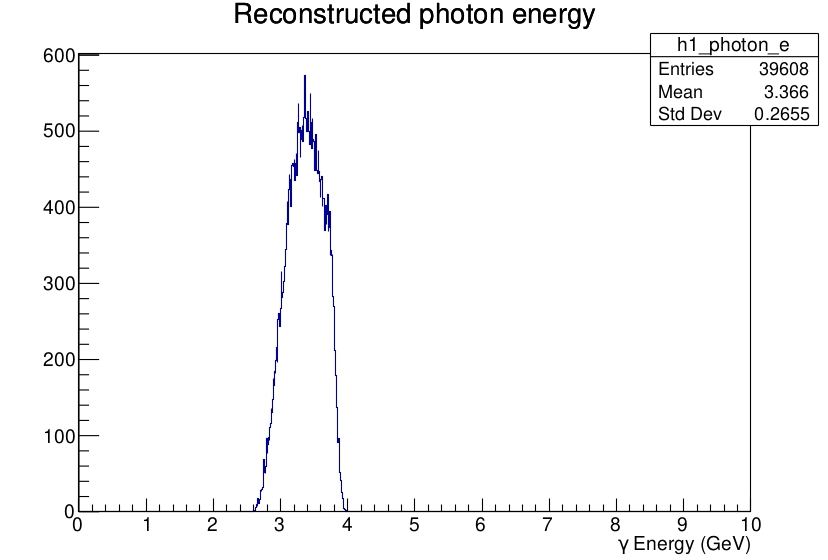
\includegraphics[scale=0.75]{Images/sbs9_hydrogen_analysis/reconstructed_photonE.png}
    \caption{Reconstructed photon energy spectrum}
    \label{fig: Reconstructed photon energy}
\end{figure}

\subsubsection{HCal active area cut}\label{HCal active area cut}
This cut selects only the $p(\gamma,\pi^+)n$ events, where the neutron \textit{would have hit} the active area of HCal, based on the $\pi^+$'s kinematics as measured by BigBite. Using the down-bending track momentum, and the reconstructed Z position of the interaction vertex in the target, we can perform a vector calculation, as we do in the GMn/nTPE analysis, to predict the hit location of the hadron in HCal, under the neutron hypothesis. If this calculation predicts the neutron to be within the active area of HCal, minus a safety margin which is set to be the dimensions of a single HCal block, the event is accepted for further analysis and if not it is discarded. This HCal active area considered is shown in Figure: \ref{fig: HCal active area}, and the effect of the HCal active area cut can be seen in the reconstructed neutron hit position distribution in Figure: \ref{fig: Reconstructed neutron hit pos on HCal}, which enforces sharp cut-offs at the left and top corners of the plot.

\begin{figure}[h!]
    \centering
    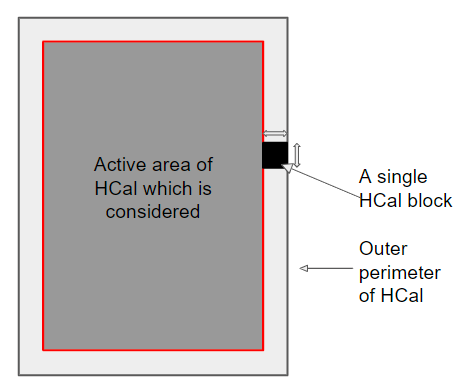
\includegraphics[scale=0.7]{Images/sbs9_hydrogen_analysis/HCal_active_areaCut.png}
    \caption{Graphical illustration of HCal active area cut}
    \label{fig: HCal active area}
\end{figure}

\begin{figure}[h!]
    \centering
    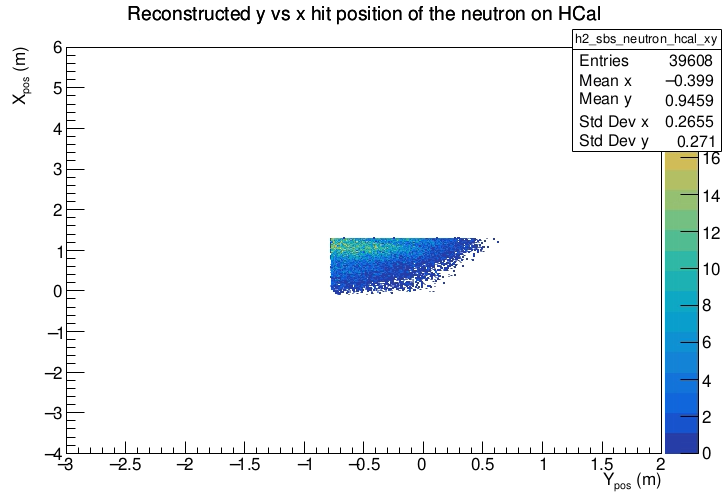
\includegraphics[scale=0.75]{Images/sbs9_hydrogen_analysis/reconstructed_neutron_hitpos_onHCal.png}
    \caption{Effect of the reconstructed neutron hit position distribution on the face of HCal, from the HCal active area cut}
    \label{fig: Reconstructed neutron hit pos on HCal}
\end{figure}
%%%%%%%%%%%%%%%%%%%%%%%%%%%%%%%%%%%%%%%%%%%%%%%%%%%%%%%%%%%%%%%%%%%%%%%%%%%%%%%%%%%%%%%%%%%%%%%%%%%%%%%%%%%%

%%%%%%%%%%%%%%%%%%%%%%%%%%%%%%%%%%%%%%%%%%%%%%%%%%%%%%%%%%%%%%%%%%%%%%%%%%%%%%%%%%%%%%%%%%%%%%%%%%%%%%%%%%%%
\subsection{Search for the ``good" neutrons in HCal from the $p(\gamma,\pi^+)n$ process}
This will essentially form the ``numerator" of the HCal neutron detection efficiency analysis. Therefore, we are allowed to use information from both the BigBite and HCal. From the side of the BigBite spectrometer, we will use all the cuts that we use for the event selection of the denominator listed in section: \ref{Denominator cuts}. From the HCal side, we will use a set of cuts that use HCal data such as ADC time, cluster position, and cluster energy, depending on the type of efficiency analysis we choose to do.

\subsubsection{Event selection cuts for the ``numerator"}\label{Numerator cuts}
The following cuts are currently being used for the event selection for numerator, or the detected good neutrons.
\begin{itemize}    
    \item HCal and BigBite shower ADC time correlation cut(Figure: \ref{fig: HCal SH ADC time corr}):
    \begin{verbatim}
        43.35 < (HCal ADC time - BigBite SH ADC time) < 59.8
    \end{verbatim}      
\end{itemize}

\begin{figure}[h!]
    \centering
    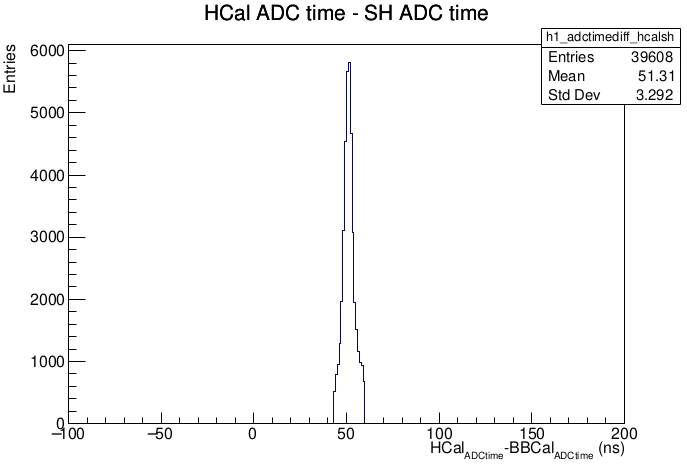
\includegraphics[scale=0.75]{Images/sbs9_hydrogen_analysis/HCalADCtime_min_SHADCtime.png}
    \caption{HCal and BigBite Shower ADC time correlation cut}
    \label{fig: HCal SH ADC time corr}
\end{figure}

%%%%%%%%%%%%%%%%%%%%%%%%%%%%%%%%%%%%%%%%%%%%%%%%%%%%%%%%%%%%%%%%%%%%%%%%%%%%%%%%%%%%%%%%%%%%%%%%%%%%%%%%%%%%%%
\subsection{``Neutron spot" plots}
These plots are being used as proof that we are seeing neutron in HCal that corresponds to the $p(\gamma,\pi^+)n$ channel. Cuts mentioned in both section: \ref{Denominator cuts} and section: \ref{Numerator cuts} were used producing these plots.\\
The main plot we can use is the so called \textit{dx vs dy} plot, which we also use a lot in the regular GMn analysis. See Figure: \ref{fig: dx vs dy} As it can be seen, there is very clearly visible neutron spot, centered around the (0,0). Another plot is to show the correlation between HCal vertical cluster position and the azimuthal angle of the $\pi^+$ as measured in BigBite. For a single channel $p(\gamma,\pi^+)n$ reaction, both the neutron and the $\pi^+$ should be in the same scattering plane and should have a tight correlation with each other's azimuthal angles. This correlation can be seen in the top left part of Figure: \ref{fig: HCalX vs phi}.

\begin{figure}[h!]
    \centering
    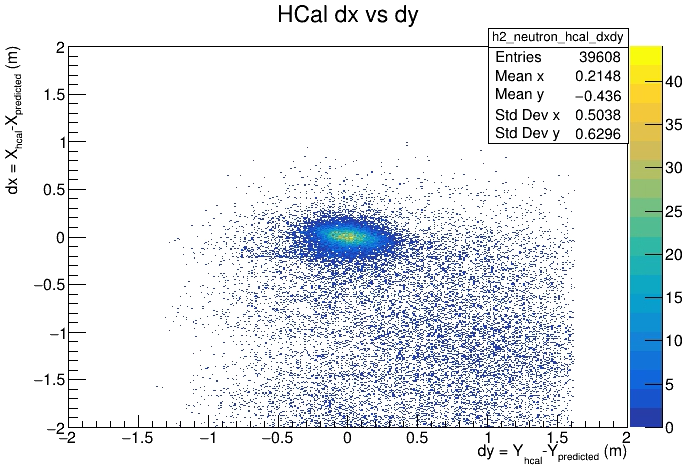
\includegraphics{Images/sbs9_hydrogen_analysis/dx_vs_dy.png}
    \caption{dx vs dy plot}
    \label{fig: dx vs dy}
\end{figure}

\begin{figure}[h!]
    \centering
    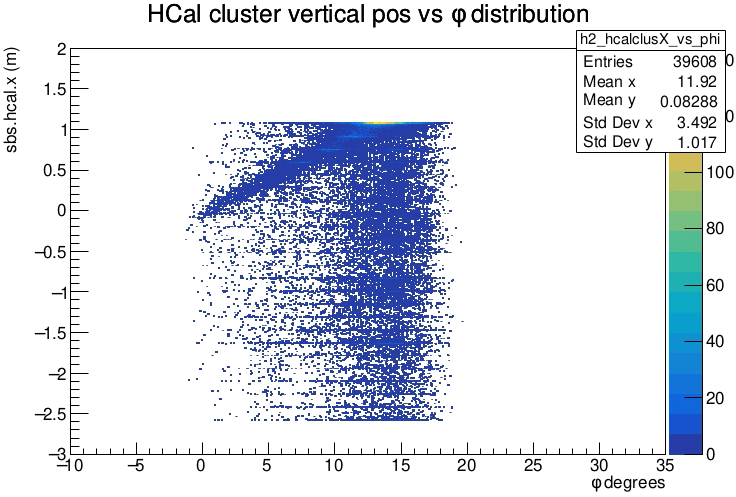
\includegraphics{Images/sbs9_hydrogen_analysis/HCalx_vs_piPhiang.png}
    \caption{HCal vertical cluster position vs the azimuthal ($\phi$) angle of the $\pi^+$}
    \label{fig: HCalX vs phi}
\end{figure}

%%%%%%%%%%%%%%%%%%%%%%%%%%%%%%%%%%%%%%%%%%%%%%%%%%%%%%%%%%%%%%%%%%%%%%%%%%%%%%%%%%%%%%%%%%%%%%%%%%%%%%%%%%%%%%
\subsection{Ideas for methods to calculate neutron detection efficiency}
Once the event selection for the denominator is completed, there could be several ways we can calculate the HCal Neutron Detection Efficiency (NDE). 

\subsubsection{``R cut" method}
This method might be the most simple method that could be implemented. The basic steps would be as follows:
\begin{enumerate}
    \item For a given denominator event, search whether the HCal cluster being considered is within a radial distance of R, from the point of expected interaction as predicted by BigBite kinematics. And also check whether the ADC time of the highest energy block of the cluster is within a tight correlation between BigBite Shower (\texttt{bb.sh.atimeblk}). 
    \begin{itemize}
        \item If yes, increment the numerator by one.
        \item If no, move on to the next event.
    \end{itemize}

    \item The ratio between the numerator from the above step and the denominator will be HCal NDE.    
\end{enumerate}

\subsubsection{By fitting a HCal  dx distribution of the neutron spot}
Another way could be to fit a HCal dx distribution with a Gaussian for the neutron peak and a polynomial for the background, which may have still passed the very tight event-selection criteria for the denominator. The background fit could also be used to further correct the denominator by subtracting the integral of the background fit from the number of events that passed through all the BB track cuts and end-point momentum cuts. The ratio of the integral of the neutron peak Gaussian fit and the corrected denominator could be interpreted as the HCal NDE.

%%%%%%%%%%%%%%%%%%%%%%%%%%%%%%%%%%%%%%%%%%%%%%%%%%%%%%%%%%%%%%%%%%%%%%%%%%%%%%%%%%%%%%%%%%%%%%%%%%%%%%%%%%%%%%
\subsection{Future plans for analyzing SBS-9 LH2 data}
\begin{itemize}
    \item Work with Andrew in PHYTHIA + g4sbs simulations to find relative pion production rates from different channels, and come up with some reasonable set of momentum cut criteria for the event selection of denominator.
    \item Resolve the issue with the momentum reconstruction of the simulated data produced using the WAAP generator. Once this is resolved, we should know better the momentum distribution of the single pion photo-production channel, which should help us to fine-tune our cut criteria in real data analysis.
\end{itemize}

%%%%%%%%%%%%%%%%%%%%%%%%%%%%%%%%%%%%%%%%%%%%%%%%%%%%%%%%%%%%%%%%%%%%%%%%%%%%%%%%%%%%%%%%%%%%%%%%%%%%%%%%%%%%%%



